% KubeEdgeInfer -- 10-slide talk in the supplied reference template.
%
% Follows the reference deck's visual language exactly: navy frame-title bars,
% rounded-and-shadowed beamer blocks, a red alertblock for the consequence, the
% WATCH/DECIDE/ACT/HEAL flow, and a tick/cross novelty table. Content covers the
% full required set of sections, so it adds a literature review, results and a
% reference list that the seven-slide reference did not carry.
%
%     latexmk -pdflatex kubeedgeinfer-classic.tex
%
% Plain pdfLaTeX is enough -- no fontspec, so this builds anywhere.

\documentclass[aspectratio=169,11pt]{beamer}

\usepackage[T1]{fontenc}
\usepackage{lmodern}
\usepackage{booktabs}
\usepackage{array}
\usepackage{pifont}       % \ding{51} tick, \ding{55} cross
\usepackage{tikz}
\usetikzlibrary{arrows.meta,positioning,calc,shadows.blur}

% ---------------------------------------------------------------- palette
% Sampled from the reference deck: one navy for all structure, one red used
% only for the consequence block, one grey for block bodies.
\definecolor{kenavy} {HTML}{1B2159}
\definecolor{kered}  {HTML}{A31D1D}
\definecolor{kegrey} {HTML}{ECECEC}
\definecolor{kegreen}{HTML}{1E7A34}

% ---------------------------------------------------------------- theme
\usetheme{default}
\setbeamertemplate{navigation symbols}{}
\setbeamercolor{structure}{fg=kenavy}
\setbeamercolor{frametitle}{fg=white,bg=kenavy}
\setbeamercolor{title}{fg=white,bg=kenavy}
\setbeamercolor{block title}{fg=white,bg=kenavy}
\setbeamercolor{block body}{bg=kegrey}
\setbeamercolor{block title alerted}{fg=white,bg=kered}
\setbeamercolor{block body alerted}{bg=kegrey}
\setbeamerfont{frametitle}{series=\bfseries}
\setbeamerfont{block title}{series=\bfseries,size=\normalsize}
% Rounded corners with a drop shadow, on both the title page and the blocks --
% the detail that gives the reference deck its look.
\setbeamertemplate{blocks}[rounded][shadow=true]
\setbeamertemplate{title page}[default][rounded=true,shadow=true]
\setbeamertemplate{itemize item}{\textbullet}
\setbeamertemplate{itemize subitem}{--}
\setbeamercolor{item}{fg=kenavy}
% Footer: page number over total, bottom right, as in the reference.
\setbeamertemplate{footline}{%
  \hfill{\tiny\insertframenumber\,/\,\inserttotalframenumber}\hspace{1.2em}%
  \vspace{0.7em}}

\newcommand{\yes}{\textcolor{kegreen}{\ding{51}}}
\newcommand{\no}{\textcolor{kered}{\ding{55}}}

\title{KubeEdgeInfer}
\subtitle{A Closed-Loop, eBPF-Driven Kubernetes Framework for Heterogeneous
          Distributed LLM Inference on Consumer Edge Clusters}
\author{Your Name}
\institute{Department of \rule{1.2cm}{0.4pt}\\Guide: Sir's Name}
\date{\today}

\begin{document}

% =============================================================== 1. Title
\begin{frame}[plain]
  \titlepage
\end{frame}

% =============================================================== 2. Introduction
\begin{frame}
  \frametitle{Introduction}
  \begin{itemize}\itemsep0.55em
    \item Large Language Models (LLMs) are often too large to fit on a single
      consumer GPU.
    \item \textbf{Pipeline parallelism} solves this by splitting model layers
      across several machines, forming an inference assembly line.
    \item Existing frameworks are built either for stable datacenter
      interconnects, or they split layers \textbf{statically} and never revisit
      that decision.
    \item Consumer and edge hardware is inherently \textbf{heterogeneous}:
      different GPU generations, WiFi rather than Ethernet, and thermal variance
      under sustained load.
  \end{itemize}
  \vfill
  \begin{block}{Core Idea}
    Continuously observe real hardware conditions at the kernel level, and let
    the model's layer partition \emph{adapt} to them instead of staying fixed.
  \end{block}
\end{frame}

% =============================================================== 3. Literature
\begin{frame}
  \frametitle{Literature Review}
  \framesubtitle{}
  \vspace{-0.4em}
  {\scriptsize
  \renewcommand{\arraystretch}{1.15}
  \begin{tabular}{@{}p{0.17\textwidth}p{0.045\textwidth}p{0.38\textwidth}p{0.33\textwidth}@{}}
    \toprule
    \textbf{Work} & \textbf{Year} & \textbf{Contribution} &
      \textbf{Gap this work addresses}\\
    \midrule
    EdgeShard & 2024 & DP device selection and layer partition &
      Profiled offline; plan never revisited\\
    Galaxy & 2024 & Tensor/sequence parallelism with overlap &
      One-shot planning, no adaptation\\
    Helix & 2025 & Max-flow MILP over mixed GPUs &
      Solver too heavy for a live loop\\
    TPI-LLM & 2024 & Memory scheduling for 70B on small RAM &
      Optimises memory, not degradation\\
    prima.cpp & 2025 & CPU/GPU co-scheduling on home clusters &
      Schedule fixed at load time\\
    Head-level split & 2025 & Attention-head granularity, with migration &
      Triggered by memory pressure only\\
    Parallax & 2025 & Serving over volunteer machines &
      No kernel-level measurement\\
    Adaptive split (MBRL) & 2025 & Learns the split point as the channel varies &
      Needs training; no optimality proof\\
    Distributed LLM survey & 2025 & Surveys the field &
      Names adaptation as an open problem\\
    sched\_ext (eBPF) & 2025 & Linux schedulers loaded as eBPF programs &
      Single host; no model pipeline\\
    \bottomrule
  \end{tabular}}
  \vfill
  \begin{block}{Common limitation}
    Every one of these measures the hardware \emph{before} the run and never
    measures again.
  \end{block}
\end{frame}

% =============================================================== 4. Problem
\begin{frame}
  \frametitle{Problem Statement}
  \vspace{0.4em}
  \textbf{Static partitioning ignores real-time hardware variability.}
  \vspace{0.9em}
  \begin{columns}[T]
  \begin{column}{0.315\textwidth}
    \begin{block}{Thermal Throttling}
      \small GPUs slow down mid-inference as they heat up under sustained load.
    \end{block}
  \end{column}
  \begin{column}{0.315\textwidth}
    \begin{block}{Network Latency}
      \small WiFi and edge links have variable latency --- no InfiniBand or
      NVLink at home.
    \end{block}
  \end{column}
  \begin{column}{0.315\textwidth}
    \begin{block}{Node Failure}
      \small A laptop closes its lid or drops off the network, and its layers
      go with it.
    \end{block}
  \end{column}
  \end{columns}
  \vfill
  \begin{alertblock}{Consequence: Pipeline Bubble Time}
    Fast machines sit idle waiting on slower ones. A one-time, fixed split
    cannot correct itself as conditions change.
  \end{alertblock}
  \vspace{0.6em}
\end{frame}

% =============================================================== 5. Contributions
\begin{frame}
  \frametitle{Objectives and Contributions}
  \begin{enumerate}\itemsep0.55em
    \item Capture system telemetry --- network transfer latency, GPU thermal
      state, throttling --- using \textbf{eBPF} and \textbf{NVML}, with no
      change to the model code.
    \item Design a \textbf{dynamic partitioning algorithm} that computes the
      optimal contiguous layer split from live telemetry, and prove it optimal
      for each snapshot.
    \item Integrate telemetry and partitioning decisions directly into a
      \textbf{Kubernetes} control loop, applying them without restarting pods.
    \item Enable \textbf{autonomous healing}: automatic re-partitioning on node
      failure or sustained thermal throttling.
    \item Stabilise the loop with \textbf{hysteresis} --- a 15\% improvement
      threshold and a 30\,s cooldown --- so noisy telemetry cannot cause
      thrashing.
    \item Evaluate bubble time, throughput and time-to-first-token empirically
      against static partitioning and an offline-profiling baseline.
  \end{enumerate}
\end{frame}

% =============================================================== 6. Architecture
\begin{frame}
  \frametitle{Architecture --- How It Works}
  \vspace{0.3em}
  \centering
  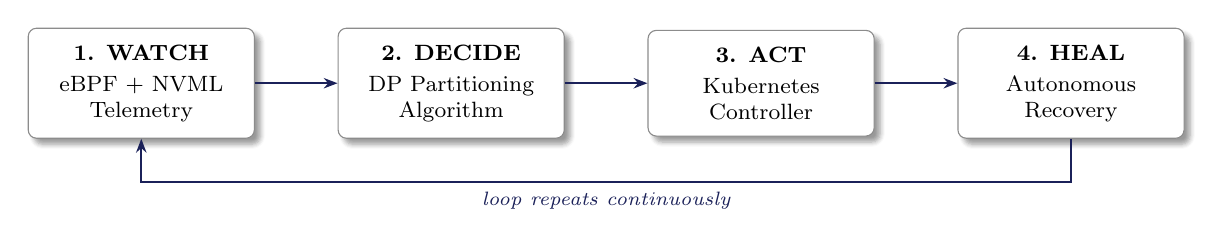
\begin{tikzpicture}[
      node distance=1.05cm,
      box/.style={draw=black!45,fill=white,rounded corners=3pt,
                  align=center,text width=2.45cm,inner sep=6pt,
                  font=\footnotesize,blur shadow={shadow blur steps=5}},
      arr/.style={-{Stealth[length=5pt]},kenavy,thick}]
    \node[box] (w) {\textbf{1. WATCH}\\[0.2em]eBPF + NVML\\Telemetry};
    \node[box,right=of w] (d) {\textbf{2. DECIDE}\\[0.2em]DP Partitioning\\Algorithm};
    \node[box,right=of d] (a) {\textbf{3. ACT}\\[0.2em]Kubernetes\\Controller};
    \node[box,right=of a] (h) {\textbf{4. HEAL}\\[0.2em]Autonomous\\Recovery};
    \draw[arr] (w) -- (d);
    \draw[arr] (d) -- (a);
    \draw[arr] (a) -- (h);
    \draw[arr] (h.south) -- ++(0,-0.55)
      -| node[pos=0.25,below,font=\scriptsize\itshape,color=kenavy]
      {loop repeats continuously} (w.south);
  \end{tikzpicture}
  \vspace{0.9em}
  \begin{itemize}\itemsep0.35em\small
    \item \textbf{Watch:} kernel-level flow latency, GPU temperature, memory,
      throttle state.
    \item \textbf{Decide:} compute the optimal contiguous split from live
      metrics.
    \item \textbf{Act:} re-assign layers, reroute traffic, apply the new split
      with no restart.
    \item \textbf{Heal:} detect node failure within 3\,s, re-partition across
      the survivors.
  \end{itemize}
\end{frame}

% =============================================================== 7. Results
\begin{frame}
  \frametitle{Results}
  \centering
  {\small
  \renewcommand{\arraystretch}{1.15}
  \begin{tabular}{@{}lccc@{}}
    \toprule
    \textbf{Injected condition} & \textbf{KubeEdgeInfer} &
      \textbf{Profile-once} & \textbf{Static split}\\
    \midrule
    No fault                 & 42\,ms & 42\,ms  & 42\,ms\\
    Thermal throttle (0.4$\times$) & \textbf{52\,ms} & 102\,ms & 102\,ms\\
    Network delay (80\,ms)   & \textbf{62\,ms} & 122\,ms & 122\,ms\\
    Thermal + network        & \textbf{62\,ms} & 182\,ms & 182\,ms\\
    Node failure             & \textbf{62\,ms} & 62\,ms  & pipeline stops\\
    \bottomrule
  \end{tabular}}
  \par\vspace{0.3em}
  {\scriptsize Bottleneck-stage cost per token; lower is better.
   12 layers over 3 machines.}
  \vfill
  \begin{block}{\normalsize Headline}
    \small\textbf{49\%} lower bottleneck cost under thermal throttling and under
    network degradation; \textbf{66\%} lower when both occur together. Under
    node failure the static split is undefined over the surviving set, so the
    pipeline stops --- KubeEdgeInfer re-partitions and continues.
  \end{block}
  \vspace{0.25em}
  {\scriptsize\itshape Reproducible with \texttt{go run ./bench/dpsim}; end-to-end
   throughput comes from \texttt{bench/run.py}, which needs a live cluster.}
\end{frame}

% =============================================================== 8. Novelty
\begin{frame}
  \frametitle{Novelty}
  \vspace{0.4em}
  \centering
  {\small
  \renewcommand{\arraystretch}{1.4}
  \begin{tabular}{@{}lccccc@{}}
    \toprule
    \textbf{Feature} & \textbf{EdgeShard} & \textbf{Galaxy} & \textbf{Helix} &
      \textbf{prima.cpp} & \textbf{Ours}\\
    \midrule
    Heterogeneous edge support   & \yes & \yes & \no  & \yes & \yes\\
    Kernel-level telemetry (eBPF)& \no  & \no  & \no  & \no  & \yes\\
    Dynamic re-partitioning      & \no  & \no  & \no  & \no  & \yes\\
    Thermal awareness            & \no  & \no  & \no  & \no  & \yes\\
    Autonomous healing           & \no  & \no  & \yes & \no  & \yes\\
    Declarative K8s API          & \no  & \no  & \no  & \no  & \yes\\
    \bottomrule
  \end{tabular}}
  \vfill
  \begin{block}{One-line novelty statement}
    We turn a static, one-time model-splitting decision into a continuous,
    self-correcting one --- driven by real kernel-level measurements instead of
    assumptions.
  \end{block}
  \vspace{0.4em}
\end{frame}

% =============================================================== 9. Summary
\begin{frame}
  \frametitle{Summary}
  \begin{itemize}\itemsep0.4em\small
    \item First system to close the loop: eBPF/NVML telemetry $\rightarrow$
      Kubernetes scheduling $\rightarrow$ self-healing, for edge LLM inference.
    \item The partitioner is \textbf{provably optimal} for a fixed telemetry
      snapshot --- it reduces to the classical linear partition problem, and is
      unit-tested against brute force on 200 random instances.
    \item Adaptive behaviour is validated \textbf{empirically} through a staged
      ablation under simulated network, thermal and failure conditions.
    \item Distributed GPT-2 output is \textbf{token-identical} to single-process
      inference, so adaptivity costs no correctness.
    \item Fully software-based and reproducible --- no proprietary hardware lab
      required.
  \end{itemize}
  \vfill
  \begin{center}
    \Large\itshape Thank you --- Questions?
  \end{center}
  \vspace{0.2em}
\end{frame}

% =============================================================== 10. References
\begin{frame}
  \frametitle{References}
  \vspace{0.3em}
  {\scriptsize
  \begin{enumerate}\itemsep0.22em
    \item M.~Zhang, J.~Cao, X.~Shen, Z.~Cui. EdgeShard: Efficient LLM Inference
      via Collaborative Edge Computing. \emph{IEEE Internet of Things Journal},
      2024. arXiv:2405.14371.
    \item Galaxy: A Resource-Efficient Collaborative Edge AI System for In-situ
      Transformer Inference. \emph{IEEE INFOCOM}, 2024. arXiv:2405.17245.
    \item Helix: Serving Large Language Models over Heterogeneous GPUs and
      Network via Max-Flow. \emph{ACM ASPLOS}, 2025. arXiv:2406.01566.
    \item TPI-LLM: Serving 70B-scale LLMs Efficiently on Low-resource Edge
      Devices. 2024. arXiv:2410.00531.
    \item Prima.cpp: Fast 30--70B LLM Inference on Heterogeneous and
      Low-Resource Home Clusters. 2025. arXiv:2504.08791.
    \item Large Language Model Partitioning for Low-Latency Inference at the
      Edge. 2025. arXiv:2505.02533.
    \item Parallax: Efficient LLM Inference Service over Decentralized
      Environment. 2025. arXiv:2509.26182.
    \item Adaptive layer splitting for wireless large language model inference
      in edge computing: a model-based reinforcement learning approach.
      \emph{FITEE}, Springer, 2025. doi:10.1631/FITEE.2400468.
    \item Distributed LLMs and Multimodal Large Language Models: A Survey on
      Advances, Challenges, and Future Directions. 2025. arXiv:2503.16585.
    \item Towards Agentic OS: An LLM Agent Framework for Linux Schedulers.
      2025. arXiv:2509.01245.
  \end{enumerate}}
  \vfill
  {\scriptsize Tools: cilium/ebpf (CO-RE loader), Kubernetes controller-runtime,
   NVIDIA NVML, k3s, Hugging Face Transformers.}
\end{frame}

\end{document}
